\documentclass{beamer}
\usepackage{ctex, hyperref}%WSL不能用ctex
\usepackage[T1]{fontenc}

% other packages
\usepackage{latexsym,amsmath,xcolor,multicol,booktabs,calligra}
\usepackage{graphicx,pstricks,listings,stackengine}
\usepackage{multicol}
\usepackage{pgf-pie}%饼图使用

\title[About Beamer]
{About the Beamer class in presentation making}
\subtitle{A short story}
\author[Eric] % (optional, for multiple authors)
{Li Guanlin\inst{1} \and J.~Doe\inst{1}}
\institute[NJU] % (optional)
{
\inst{1}%
Undergraduates of ICS\\
Nanjing University
\and
% \inst{2}%
% Faculty of Chemistry\\
% Very Famous University
}
\date[NJU 2023] % (optional)
{\today}
\usepackage{NJU}

% defs
\def\cmd#1{\texttt{\color{red}\footnotesize $\backslash$#1}}
\def\env#1{\texttt{\color{blue}\footnotesize #1}}
\definecolor{deepblue}{rgb}{0,0,0.5}
\definecolor{deepred}{rgb}{0.6,0,0}
\definecolor{deepgreen}{rgb}{0,0.5,0}
\definecolor{halfgray}{gray}{0.55}

\lstset{
    basicstyle=\ttfamily\small,
    keywordstyle=\bfseries\color{deepblue},
    emphstyle=\ttfamily\color{deepred},    % Custom highlighting style
    stringstyle=\color{deepgreen},
    numbers=left,
    numberstyle=\small\color{halfgray},
    rulesepcolor=\color{red!20!green!20!blue!20},
    frame=shadowbox,
}

\renewcommand{\familydefault}{\rmdefault} %可选择\rmdefault \sfdefault \ttdefault 分别是罗马字体,sans-serif字体和等宽字体  \familydefault是默认字体

\begin{document}

\begin{frame}
    \titlepage
    \begin{figure}[htpb]
        \begin{center}
            
\includegraphics[width=0.2\linewidth]{pic/NJU_Logo.eps}
        \end{center}
    \end{figure}
\end{frame}

\begin{frame}
    \tableofcontents[sectionstyle=show,subsectionstyle=show/shaded/hide,subsubsectionstyle=show/shaded/hide]
\end{frame}

\section{Introduction}
\subsection{Starters}
\begin{frame}
    \frametitle{Introduction}
    \Large
    \begin{itemize}[<+->]
        \item Lots of career planning classes
        \item Heard of the importance of career planning
        \item Many people attach great importance to it
    \end{itemize}
    \onslide<4>
    \begin{center}
        \LARGE
        \textbf{Dose it really work?} 
    \end{center}
\end{frame}

\subsection{Info}
\begin{frame}
    \frametitle{Study Question}
    \Huge
    \begin{center}
        \textbf{Is career planing really correlated with academic success?}        
    \end{center}
\end{frame}

\begin{frame}
    \frametitle{Significance}  
    \Large
    \begin{itemize}
        \item Discover the relationship between career planning and academic success
        \item Help students to understand whether it is important to have career planning
    \end{itemize}
\end{frame}

\section{Methods}
\begin{frame}
    \frametitle{Methods}
    \LARGE
    \begin{itemize}[<+->]
        \item Literature study
        \item Send Questionnaire
        \item Data analysis
    \end{itemize}
\end{frame}

\subsection{Survey}
\subsubsection*{Sample Size}

\begin{frame}
    \frametitle{Sample Size}
    \LARGE
    \begin{center}
        Valid Questionnaires: 40

        Total Questionnaires: 42
    \end{center}
\end{frame}

\subsubsection*{Questionnaire Design}
\begin{frame}
    \frametitle{Evaluation of Career Planing}
    \begin{enumerate}
        \item [1] Have you ever thought about what kind of occupation you want to go in for in the future?(eg. I want to pursue a career in biology, physics or linguistics)
        \item [2] You feel that your planning is manageable and doable. Besides, you are confident on the career planning and will not give up in a short period of time. (eg.some students major in bioengineering are quite confused with their future planning)
        \item [3]You know exactly what you are eager to do and is able to generalize what it is in one sentence or you have no idea about the specific jobs but have a sketch of what to do in the future (eg.I want to be a police to successfully thwart a gang of drug traffickers)
    \end{enumerate}
\end{frame}

\begin{frame}
    \frametitle{Evaluation of Career Planing}
    \begin{enumerate}
        \item [4] You’re considerably clear about what skills you should grasp so as to achieve your goal
        \item [5] In order to grasp those skills discussed above, you have a well-planned scheme of learning (eg. I have to grasp A in this semester or have a proficient command of B in the duration of your undergraduate stage)
        \item [6] The learning scheme mentioned above has become an indispensable part of your daily life, which makes you energetic and have a sense of fulfillment as well as getting closer to your target.
    \end{enumerate}
\end{frame}

\begin{frame}
    \frametitle{Evaluation of Academic Performance}
    \begin{enumerate}
        \item [7] Objectively speaking, if asked to grade yourself according to your academic performance, which choice below is the best one that conforms to your self-estimation?:
        \begin{itemize}
            \item [A] Excellent, I’m the king.
            \item [B] Good enough but not perfect
            \item [C] Not that good but acceptable
            \item [D] There is a long way to go
            \item [E] Terrible, I don’t want to mention that
            \item [F] Sorry, life is hard 
        \end{itemize}
    \end{enumerate}
\end{frame}

\section{Results}
\subsection{Conclusion of the Previous Studies}
\begin{frame}
    \frametitle{Conclusion of Previous Studies}
    \large
    \begin{itemize}[<+->]
        \item Self-efficacy expectations are related to indices of academic performance behavior as well as vocational interest and range of perceived career options.\cite{lent1986self}
        \item A career planing course does have a positive impact on academic performance.\cite{folsom2005impact}
        \item A systematric advisement system would enhance opportunities for student academic success.\cite{jones1983impact}
    \end{itemize}
\end{frame}

\subsection{Results of the Survey}
\begin{frame}
    \frametitle{Horizontal contrast}
    \tiny
    \begin{figure}[htbp]
        \centering
        \begin{minipage}[t]{0.4\textwidth}
            \centering
            % \raggedleft
            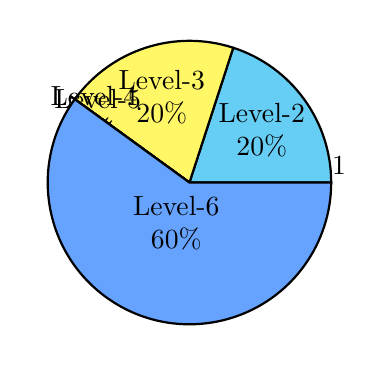
\begin{tikzpicture}
                \pie[text=inside,explode={0, 0, 0, 0.1},scale=0.6]{0/Level-1,20/Level-2, 20/Level-3, 0/Level-4, 0/Level-5, 60/Level-6}
            \end{tikzpicture}
            \caption{Excellent, I’m the king} \label{fig:pie1}
        \end{minipage}
        \begin{minipage}[t]{0.4\textwidth}
            \centering
            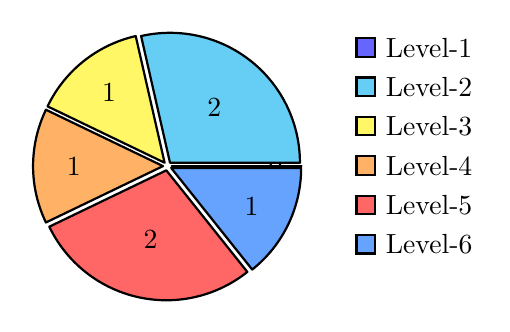
\begin{tikzpicture}
                \pie[text=legend,explode=0.1,scale=0.55,sum=auto]{0/Level-1,2/Level-2, 1/Level-3, 1/Level-4, 2/Level-5, 1/Level-6}
            \end{tikzpicture}
            \caption{Good enough but not perfect} \label{fig:pie2}
        \end{minipage}
    \end{figure}
\end{frame}

\begin{frame}
    \frametitle{Horizontal contrast}
    \tiny
    \begin{figure}[htbp]
        \centering
        \begin{minipage}[t]{0.4\textwidth}
            \centering
            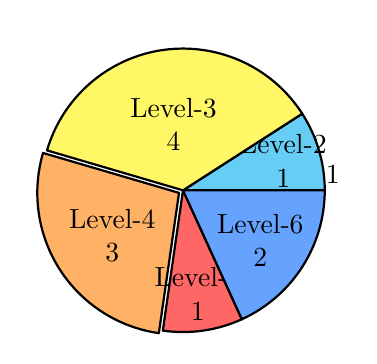
\begin{tikzpicture}
                \pie[text=inside,explode={0, 0, 0, 0.1},scale=0.6,sum=auto]{0/Level-1,1/Level-2, 4/Level-3, 3/Level-4, 1/Level-5, 2/Level-6}
            \end{tikzpicture}
            \caption{Not that good but acceptable}\label{fig:pie3}
        \end{minipage}
        \begin{minipage}[t]{0.4\textwidth}
            \centering
            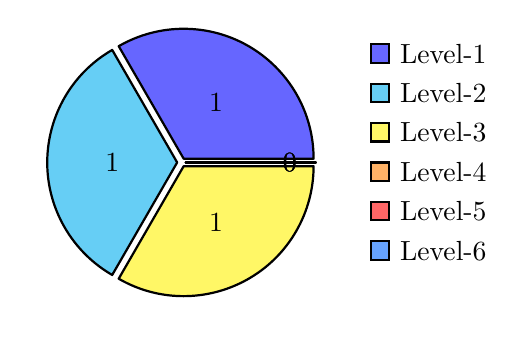
\begin{tikzpicture}
                \pie[text=legend,explode=0.1,scale=0.55,sum=auto]{1/Level-1,1/Level-2, 1/Level-3, 0/Level-4, 0/Level-5, 0/Level-6}
            \end{tikzpicture}
            \caption{There is a long way to go}\label{fig:pie4}
        \end{minipage}
    \end{figure}
\end{frame}

\begin{frame}
    \frametitle{Horizontal contrast}
    \tiny
    \begin{figure}[htbp]
        \centering
        \begin{minipage}[t]{0.4\textwidth}
            \centering
            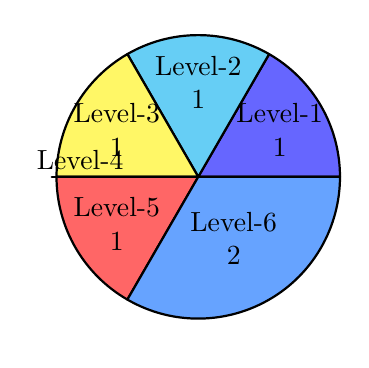
\begin{tikzpicture}
                \pie[text=inside,explode={0, 0, 0, 0.1},scale=0.6,sum=auto]{1/Level-1,1/Level-2, 1/Level-3, 0/Level-4, 1/Level-5, 2/Level-6}
            \end{tikzpicture}
            \caption{Terrible, I don’t want to mention that}\label{fig:pie5}
        \end{minipage}
        \begin{minipage}[t]{0.4\textwidth}
            \centering
            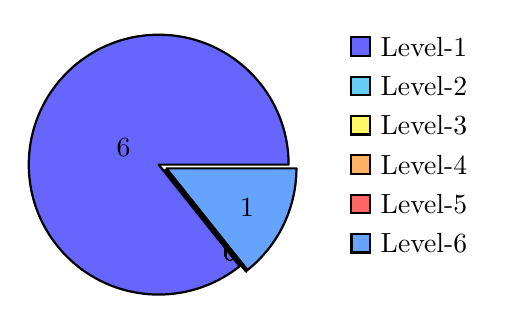
\begin{tikzpicture}
                \pie[text=legend,explode=0.1,scale=0.55,sum=auto]{6/Level-1,0/Level-2, 0/Level-3, 0/Level-4, 0/Level-5, 1/Level-6}
            \end{tikzpicture}
            \caption{Sorry, life is hard} \label{fig:pie6}
        \end{minipage}
    \end{figure}
\end{frame}

\begin{frame}
    \frametitle{Longitudinal contrast}
    \begin{figure}[htbp]
        \centering
        \begin{minipage}[t]{0.4\textwidth}
            \centering
            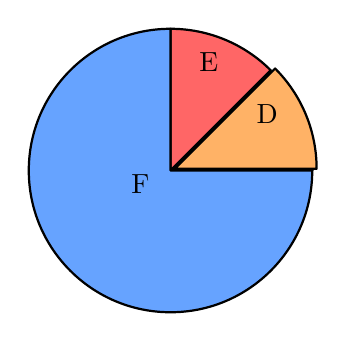
\begin{tikzpicture}
                \pie[text=inside,explode={0, 0, 0, 0.1},scale=0.6,sum=auto,hide number]{0/A, 0/B, 0/C, 1/D, 1/E, 6/F}
            \end{tikzpicture}
            \caption{Level-1} \label{fig:pie7}
        \end{minipage}
        \begin{minipage}[t]{0.4\textwidth}
            \centering
            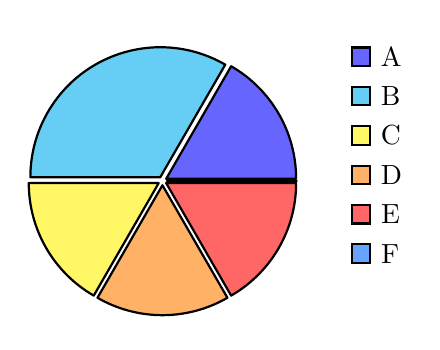
\begin{tikzpicture}
                \pie[text=legend,explode=0.1,scale=0.55,sum=auto,hide number]{1/A, 2/B, 1/C, 1/D, 1/E, 0/F}
            \end{tikzpicture}
            \caption{Level-2} \label{fig:pie8}
        \end{minipage}
    \end{figure}
\end{frame}

\begin{frame}
    \frametitle{Longitudinal contrast}
    \begin{figure}[htbp]
        \centering
        \begin{minipage}[t]{0.4\textwidth}
            \centering
            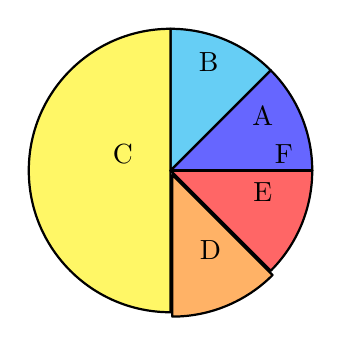
\begin{tikzpicture}
                \pie[text=inside,explode={0, 0, 0, 0.1},scale=0.6,sum=auto,hide number]{1/A, 1/B, 4/C, 1/D, 1/E, 0/F}
            \end{tikzpicture}
            \caption{Level-3} \label{fig:pie9}
        \end{minipage}
        \begin{minipage}[t]{0.4\textwidth}
            \centering
            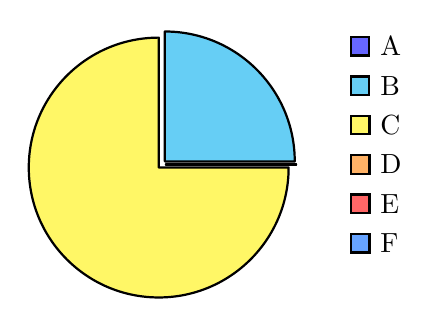
\begin{tikzpicture}
                \pie[text=legend,explode=0.1,scale=0.55,sum=auto,hide number]{0/A, 1/B, 3/C, 0/D, 0/E, 0/F}
            \end{tikzpicture}
            \caption{Level-4} \label{fig:pie10} 
        \end{minipage}
    \end{figure}
\end{frame}

\begin{frame}
    \frametitle{Longitudinal contrast}
    \begin{figure}[htbp]
        \centering
        \begin{minipage}[t]{0.4\textwidth}
            \centering
            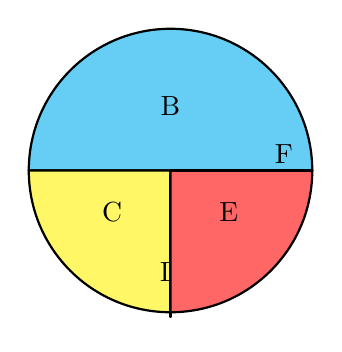
\begin{tikzpicture}
                \pie[text=inside,explode={0, 0, 0, 0.1},scale=0.6,sum=auto,hide number]{0/A, 2/B, 1/C, 0/D, 1/E, 0/F}
            \end{tikzpicture}
            \caption{Level-5} \label{fig:pie11}
        \end{minipage}
        \begin{minipage}[t]{0.4\textwidth}
            \centering
            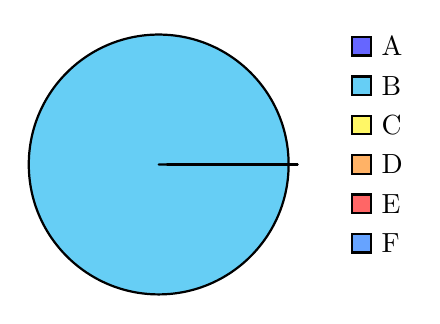
\begin{tikzpicture}
                \pie[text=legend,explode=0.1,scale=0.55,sum=auto,hide number]{0/A, 1/B, 0/C, 0/D, 0/E, 0/F}
            \end{tikzpicture}
            \caption{Level-6} \label{fig:pie12}
        \end{minipage}
    \end{figure}
\end{frame}

\subsection{Results Analysis}
\begin{frame}
    \frametitle{Horizontal Analysis}
    \Large
    \begin{itemize}[<+->]
        \item In \Cref{fig:pie1}, top students are highly possible to have a good career plan.
        \item In \Cref{fig:pie6}, the students who are not good at study are not good at career plan either.
        \item In \Cref{fig:pie2,fig:pie3,fig:pie4,fig:pie5}, the students in the middle do not show a clear tendency.
    \end{itemize}
\end{frame}

\begin{frame}
    \frametitle{Vertical Analysis}
    \Large
    \begin{itemize}
        \item In \Cref{fig:pie7}, the students with the worst career planing perform poorly in academic.
        \item In \Cref{fig:pie8,fig:pie9}, there is no obvious tendency.
        \item In \Cref{fig:pie10,fig:pie11,fig:pie12}, the students with the best career planing perform pretty well in academic.
    \end{itemize}
\end{frame}

\section{Discussion}
\begin{frame}
    \frametitle{Discussion}
    \LARGE
    \begin{itemize}[<+->]
        \item No Inferiority
        \item No Superiority
        \item A Good Choice (hope and motivation)
        \item Reconsider
    \end{itemize}
\end{frame}

\section{References}

\begin{frame}[allowframebreaks]
    \bibliography{ref}
    \bibliographystyle{acm}
    % 如果参考文献太多的话,可以像下面这样调整字体:
    % \tiny\bibliographystyle{alpha}
\end{frame}

\begin{frame}
    \begin{center}
        {\Huge\calligra Thanks!}\cite{origin}
    \end{center}
\end{frame}

\end{document}